%% Chapter 15 — Intellectual Property Basics
%% Course 247-519-VA, Vanier College
%% Project Planning & Prototyping

\chapter{Intellectual Property Basics}
\label{ch15}

\paragraph{Where this fits.}
Chapter~14 validated that the IoT robotic sorting subsystem performs as specified
--- sensors confirmed, firmware tested, Gate~3 acceptance criteria met.
Before that validated design is shown to an external manufacturer, presented at a
trade show, or handed to a licensing partner, a different question must be
answered: \emph{who owns what, and how is it protected?}
This chapter addresses that question.
It introduces the four main categories of \textbf{intellectual property}\index{intellectual property}
protection available to engineering teams, explains how ownership is determined in
employment and contract relationships, and establishes the procedural habits ---
NDAs, prior-art searches, timely filings --- that separate teams that retain the
value of their innovations from those that accidentally surrender it.

\paragraph{Learning Objectives.}
After completing this chapter you will be able to:
\begin{enumerate}
  \item Distinguish the four main types of IP protection and state what each covers.
  \item Explain IP ownership in an employment context and identify what your contract determines.
  \item Recognise when an NDA is required and what it does and does not protect.
  \item Identify the IP considerations relevant to your prototype and know when to consult a lawyer.
\end{enumerate}

A working prototype is an achievement.
It is also, depending on what it contains, a liability if it is shown to the wrong
person at the wrong moment without the right paperwork in place.
The sensor array your team spent three months tuning, the inference algorithm that
runs at a tenth of the compute budget of any comparable product, the trained model
weights --- none of these are automatically protected simply because your team
created them.
Protection is an active choice, made at specific moments in the development
timeline, governed by specific legal instruments.
This chapter gives you the vocabulary and the procedural awareness to make those
choices deliberately rather than by accident.

% ─────────────────────────────────────────────────────────────────────────────
\section{Why IP Matters to Technicians}
\label{sec:ch15-why}
% ─────────────────────────────────────────────────────────────────────────────

\index{intellectual property!relevance to technicians}The prototype you build may
be your employer's most valuable asset.
The firmware you write at Stage~3 encodes design decisions that took months to
converge.
The sensor calibration routine that eliminates thermal drift is not obvious --- it
is the product of systematic experimentation and may be genuinely novel.
The BOM you assembled, the supplier relationships you established, and the test
data you collected all have economic value that persists long after the prototype
has been demonstrated.

IP law exists to provide a framework for capturing and defending that value.
It does so imperfectly --- enforcement is expensive, international coverage is
fragmented, and small teams rarely have the resources to litigate.
But the framework also creates \emph{presumptive rights} that are cheap to
establish and expensive to ignore.
A provisional patent application filed for a few hundred dollars before a
conference presentation preserves a filing date that cannot be recovered after the
fact.
An NDA signed before showing a prototype to a contract manufacturer costs nothing
but fifteen minutes; the absence of that signature can cost everything.

Understanding IP is not a specialisation for lawyers.
It is a baseline competency for anyone who creates things that other people might
want to copy, license, or claim as their own.

% ─────────────────────────────────────────────────────────────────────────────
\section{Types of IP Protection}
\label{sec:ch15-types}
% ─────────────────────────────────────────────────────────────────────────────

Figure~\ref{fig:ch15-ip-types} summarises the four main categories of IP
protection across four attributes.
Each category covers a different kind of creative or commercial asset, operates
through a different legal mechanism, and involves a different set of trade-offs.

\begin{figure}[htbp]
  \centering
  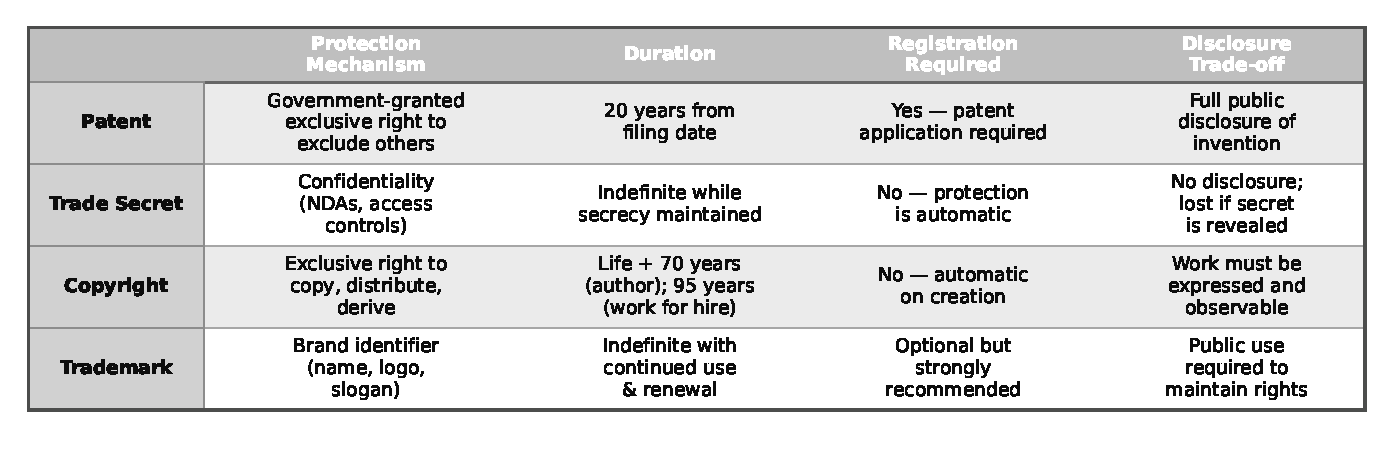
\includegraphics[width=0.92\textwidth]{chapters/15-ip/images/fig_01_ip_types}
  \caption{Comparison of the four main IP protection categories across key
           attributes.
           Duration and registration requirements differ substantially across
           categories; the right choice depends on what is being protected and
           how long secrecy versus exclusivity serves the business.}
  \label{fig:ch15-ip-types}
\end{figure}

\subsection{Patents}
\label{subsec:ch15-patents}

\index{patent}\index{patent!utility}A \textbf{patent} grants its holder the
exclusive right to make, use, sell, and import a claimed invention for a fixed
period --- twenty years from the filing date for a utility patent in Canada and
the United States.
In exchange for that exclusivity, the inventor discloses the invention fully and
publicly.
This is the fundamental trade-off of the patent system: a temporary monopoly in
exchange for permanent public knowledge.

For a patent to be granted, the claimed invention must satisfy three criteria.
\textbf{Novelty}\index{patent!novelty}: the invention must not have been publicly
disclosed before the priority date.
\textbf{Non-obviousness}\index{patent!non-obviousness} (``inventive step'' in
Canadian and European terminology): the invention must not be an obvious extension
of what a person skilled in the relevant field would already know.
\textbf{Utility}\index{patent!utility}: the invention must have a specific,
credible, and substantial use.

\index{provisional patent application}A \textbf{provisional patent application}
is a lower-cost, lower-formality filing that establishes a priority date without
beginning the examination process.
It expires after twelve months unless a full (non-provisional) application is
filed.
For engineering teams at the prototype stage, a provisional application is the
most practical instrument for preserving patent rights before a public disclosure
--- a conference presentation, a trade-show demonstration, or a publication ---
that would otherwise destroy novelty.

\subsection{Trade Secrets}
\label{subsec:ch15-trade-secrets}

\index{trade secret}A \textbf{trade secret} is any information that (a) derives
economic value from not being generally known, (b) is not readily ascertainable
by others who could benefit from it, and (c) is subject to reasonable steps to
maintain its secrecy.
Unlike a patent, a trade secret requires no registration and involves no
disclosure.
Protection is indefinite --- provided the secret remains secret.

The critical phrase is ``reasonable steps.''
Courts have found that trade secret protection is lost when the holder fails to
implement basic confidentiality controls: access logging, need-to-know
restrictions, confidentiality clauses in employment agreements, and NDAs with
external parties.
A company that leaves its training dataset on a shared drive without access
controls and then tries to sue a departing employee for misappropriation will find
that its trade secret claim is difficult to sustain.

The strategic alternative to a trade secret is a patent.
The choice is not always obvious.
A patent provides clear, enforceable rights but requires disclosure and expires.
A trade secret provides indefinite protection but can be lost to independent
discovery, reverse engineering (where permitted), or simple carelessness.
For formulas, algorithms, and processes that cannot be reverse-engineered from
the product --- the canonical example is the Coca-Cola formula --- the trade
secret may be the superior instrument.
For hardware geometries or circuit topologies that a skilled engineer could deduce
from a production unit, a patent is usually preferable.

\subsection{Copyright}
\label{subsec:ch15-copyright}

\index{copyright}\textbf{Copyright} protects original works of authorship fixed
in a tangible medium.
In engineering contexts this includes firmware source code, schematic files, PCB
layout files, simulation scripts, test harnesses, documentation, and this
textbook.
Copyright arises \emph{automatically at the moment of creation} --- no
registration, no notice, no filing.
In Canada and the United States, the term for a work created by an individual
author is the life of the author plus seventy years.

Copyright protects the \emph{expression}, not the underlying idea.
Two engineers can independently write firmware that performs the same function;
copyright does not prevent that.
What copyright prevents is one engineer copying the other's \emph{source file}
and redistributing it as their own.
This distinction --- idea versus expression --- is fundamental and frequently
misunderstood.

\index{work made for hire}\index{copyright!work made for hire}In an employment
context, firmware and documentation created by an employee in the scope of their
employment is typically a \textbf{work made for hire}, meaning the employer, not
the employee, is the legal author and first copyright owner.
In a contracting context, the situation is less clear and must be addressed
explicitly in the contract (see Section~\ref{sec:ch15-contract}).

\subsection{Trademarks}
\label{subsec:ch15-trademarks}

\index{trademark}A \textbf{trademark} is a word, name, symbol, design, or
combination thereof that identifies the source of goods or services and
distinguishes them from competitors'.
Trademark rights arise from \emph{use in commerce} --- a mark in active, public
commercial use acquires common-law protection in the geographic area where it is
used, regardless of registration.
Registration with the Canadian Intellectual Property Office (CIPO) or the United
States Patent and Trademark Office (USPTO) provides additional benefits: national
constructive notice, the right to use the \textregistered\ symbol, and a stronger
foundation for international filings.

For a team at the prototype stage, trademark questions are secondary to patent and
trade-secret questions.
The product has not yet launched commercially, so there is no use in commerce.
However, selecting a product name early --- and verifying that it does not conflict
with an existing registered mark in the target market --- avoids a costly rebrand
after investment has been made in packaging, labelling, and marketing materials.

% ─────────────────────────────────────────────────────────────────────────────
\section{IP Ownership in Employment}
\label{sec:ch15-ownership}
% ─────────────────────────────────────────────────────────────────────────────

\index{IP ownership!employment}\index{employment agreement}The default rule in
most common-law jurisdictions is that inventions and creative works produced by an
employee \emph{within the scope of their employment} belong to the employer, not
the employee.
This rule applies even when the work is performed at home, outside normal hours,
using personal equipment --- provided the work relates to the employer's business
or uses information or resources to which the employee had access through the
employment relationship.

The \textbf{employment agreement}\index{employment agreement!IP clause} modifies
this default and is the document that actually determines ownership in most
disputes.
A well-drafted employment agreement will include:
\begin{itemize}
  \item an \emph{IP assignment clause} assigning to the employer all inventions
        and works related to the employer's business, whether created during or
        after working hours;
  \item a \emph{prior inventions schedule} in which the employee lists inventions
        they created before employment that they wish to retain; and
  \item a \emph{non-compete and non-solicitation clause} restricting what the
        employee may do for a defined period after leaving.
\end{itemize}

\index{scope of employment}The phrase \textbf{scope of employment} is the
battleground in most disputes.
Courts apply a multi-factor test that includes: whether the work was the type the
employee was hired to perform; whether the work occurred substantially within
authorised hours and space; and whether the work was motivated, at least in part,
by a purpose to serve the employer.
A technician hired to develop IoT firmware who writes, on a personal laptop on a
Sunday, a sensor driver that solves a problem the team has been trying to solve for
three weeks, will find it very difficult to claim personal ownership of that driver.
The work falls squarely within the scope of employment regardless of when and where
it was performed.

The practical guidance is simple: read your employment agreement before you start
working.
If there is no prior inventions schedule and you have pre-existing IP you wish to
retain, negotiate its inclusion before signing.
After you have started working, the opportunity to carve out personal inventions
from the employer's claims becomes much narrower.

% ─────────────────────────────────────────────────────────────────────────────
\section{Non-Disclosure Agreements}
\label{sec:ch15-nda}
% ─────────────────────────────────────────────────────────────────────────────

\index{NDA}\index{non-disclosure agreement}A \textbf{non-disclosure agreement}
(NDA) --- also called a \textbf{confidentiality agreement}\index{confidentiality
agreement} --- is a contract in which one or both parties agree not to disclose
specified confidential information to third parties.
An NDA is the primary instrument for sharing a design with an external party ---
a contract manufacturer, a supplier, a potential investor, an academic advisor ---
without sacrificing trade-secret protection or triggering the novelty clock on a
patent application.

A well-drafted NDA for an engineering prototype exchange typically includes:
\begin{enumerate}
  \item \textbf{Definition of confidential information.}
        Specify precisely what is covered: technical drawings, firmware source
        code, training datasets, BOM details, and performance data.
        Overly broad definitions (``all information exchanged'') can be
        unenforceable; overly narrow definitions leave gaps.
  \item \textbf{Permitted uses.}
        State explicitly what the receiving party may do with the information
        --- evaluate it for a potential contract, quote on manufacturing, provide
        engineering feedback --- and what they may not do --- share it with
        subcontractors without consent, use it for their own competing development.
  \item \textbf{Term and survival.}
        Specify how long the obligation lasts and which obligations survive
        termination of the agreement (typically the confidentiality obligations
        themselves).
  \item \textbf{Exclusions.}
        Standard exclusions include information that was already publicly known,
        information independently developed by the receiving party, and information
        received from a third party without restriction.
\end{enumerate}

What an NDA does \emph{not} protect is equally important to understand.
An NDA does not give you a patent.
If the receiving party independently develops the same invention without using your
confidential information, the NDA provides no remedy.
An NDA does not protect information that is already in the public domain --- if
you disclosed your design at a conference last month without a patent filing, the
NDA you sign this month cannot retroactively un-disclose it.
An NDA also does not prevent a receiving party from hiring your employees and
acquiring the knowledge through them, unless the NDA is coupled with an
appropriate non-solicitation clause.

% ─────────────────────────────────────────────────────────────────────────────
\section{IP Assignment in Contract Work}
\label{sec:ch15-contract}
% ─────────────────────────────────────────────────────────────────────────────

\index{IP assignment!contract work}\index{contractor IP}When a company engages an
independent contractor to perform design work, the default IP ownership rule
differs from the employment rule.
In most common-law jurisdictions, an independent contractor retains ownership of
work product unless an explicit written assignment transfers those rights to the
client.
This reverses the employment default and catches many companies by surprise.

A contract that says ``the contractor will design a custom sensor interface PCB
for \$8,000'' says nothing about who owns the resulting schematic, firmware, or
any patentable improvement embedded in the design.
Without an explicit assignment, the contractor owns all of it.
The client has, at best, an implied licence to use the specific deliverable for
the specific purpose contracted --- not a right to modify it, not a right to have
it manufactured by a different vendor, and certainly not a right to patent it.

The remedy is a clear \textbf{IP assignment clause}\index{IP assignment clause}
in the contract, negotiated before work begins, that assigns to the client all
rights in the work product, including any inventions, copyrights, and moral
rights.
The contract should also address:
\begin{itemize}
  \item \emph{Background IP}: technology the contractor brings to the engagement
        that pre-exists the contract.
        The contractor typically retains this; the client receives a licence to
        use it only as embedded in the deliverable.
  \item \emph{Foreground IP}: new inventions and works created specifically for
        the engagement.
        This is what the assignment clause transfers.
  \item \emph{Third-party IP}: open-source libraries, licensed components, and
        third-party toolchains embedded in the deliverable.
        The client needs to understand the licence terms for everything that ships.
\end{itemize}

The time to negotiate IP ownership is before the statement of work is signed, not
after the prototype is demonstrated.
After delivery, the contractor has received payment and has no incentive to grant
additional rights; the client has expended engineering resources on a design it
may not legally be able to commercialise.

% ─────────────────────────────────────────────────────────────────────────────
\section{The Prior-Art Search}
\label{sec:ch15-prior-art}
% ─────────────────────────────────────────────────────────────────────────────

\index{prior art}\index{prior-art search}A \textbf{prior-art search} is a
systematic review of publicly available documents --- patents, published patent
applications, academic papers, product specifications, conference proceedings ---
to determine whether an invention is novel before committing to a design direction
or filing a patent application.
Conducting a prior-art search early avoids investing significant engineering
resources in a direction that is already patented, teaches design-around
opportunities, and provides the technical background that a patent attorney will
require when drafting claims.

The primary search tools available without cost are:
\begin{itemize}
  \item \textbf{Google Patents} (\texttt{patents.google.com}): full-text search
        across US, European, PCT, and many national patent databases, with
        machine-translation support for non-English documents.
  \item \textbf{USPTO Patent Full-Text Database} (\texttt{patents.uspto.gov}):
        authoritative for US filings; supports classification-based searches
        using the Cooperative Patent Classification (CPC) system.
  \item \textbf{Espacenet} (\texttt{worldwide.espacenet.com}): the European
        Patent Office's database, covering over 130 million documents from
        100-plus countries.
  \item \textbf{CIPO Patent Database} (\texttt{brevets-patents.ic.gc.ca}):
        the Canadian Intellectual Property Office's searchable database for
        Canadian filings.
\end{itemize}

\index{patent classification}Effective searching combines keyword searches with
\textbf{classification-based searches} using the CPC.
A keyword search for ``sensor array classification neural network'' will return
many irrelevant results; a search limited to CPC subclass G06N~3 (neural network
computing) and G01D~5 (measuring instruments, sensor arrays) is far more targeted.

The output of a prior-art search for the portfolio entry in Section~\ref{sec:ch15-portfolio}
should include: the databases searched, the search terms and classification codes
used, a list of the most relevant documents found, and a brief assessment of how
the invention differs from each.
This record serves two purposes: it demonstrates due diligence, and it becomes the
starting point for a patent attorney's more thorough patentability opinion.

% ─────────────────────────────────────────────────────────────────────────────
\section{When to Ask a Lawyer}
\label{sec:ch15-lawyer}
% ─────────────────────────────────────────────────────────────────────────────

\index{patent attorney}\index{legal counsel}This chapter provides
\emph{professional literacy}, not legal advice.
The distinction matters.
Professional literacy means you can identify that a situation raises an IP issue,
describe it accurately, and ask the right questions.
Legal advice means a qualified professional analyses the specific facts, applies
the applicable law, and tells you what to do.
The two are not interchangeable.

The situations that require a \textbf{patent agent} or \textbf{patent attorney}
include:
\begin{itemize}
  \item Drafting and filing a patent application.
        Claims drafting is a specialised skill; poorly drafted claims can leave
        large gaps in protection that competitors will exploit.
  \item Evaluating a freedom-to-operate opinion before commercialising a product.
        A freedom-to-operate (FTO) analysis determines whether your product would
        infringe any valid, enforceable patent in the target markets.
  \item Responding to a cease-and-desist letter or an office action from a
        patent office.
  \item Negotiating an IP licence agreement or a technology transfer agreement.
\end{itemize}

The situations that you can handle with professional literacy --- but should
escalate if ambiguous --- include:
\begin{itemize}
  \item Recognising that a disclosure event is approaching and ensuring a
        provisional patent application is filed or NDAs are in place beforehand.
  \item Reviewing a standard NDA for the four elements described in
        Section~\ref{sec:ch15-nda} and flagging missing or unusual provisions.
  \item Identifying which elements of a design may be protectable and preparing
        a structured description for the attorney's review.
  \item Confirming that an employment or contractor agreement includes an explicit
        IP assignment clause.
\end{itemize}

The earlier an attorney is engaged, the less expensive the engagement tends to be.
A brief consultation at Stage~2 to advise on patentability and filing strategy
costs far less than attempting to correct a defective filing or recover from an
invalidating disclosure after the fact.

% ─────────────────────────────────────────────────────────────────────────────
\subsection{Worked Example --- IP Audit for the Running Example}
\label{subsec:ch15-worked}
% ─────────────────────────────────────────────────────────────────────────────

\index{worked example!IP audit}Figure~\ref{fig:ch15-ip-timeline} maps the IP
considerations for the IoT robotic sorting subsystem across the Stage-Gate
timeline.
The following audit applies each category in turn.

\begin{figure}[htbp]
  \centering
  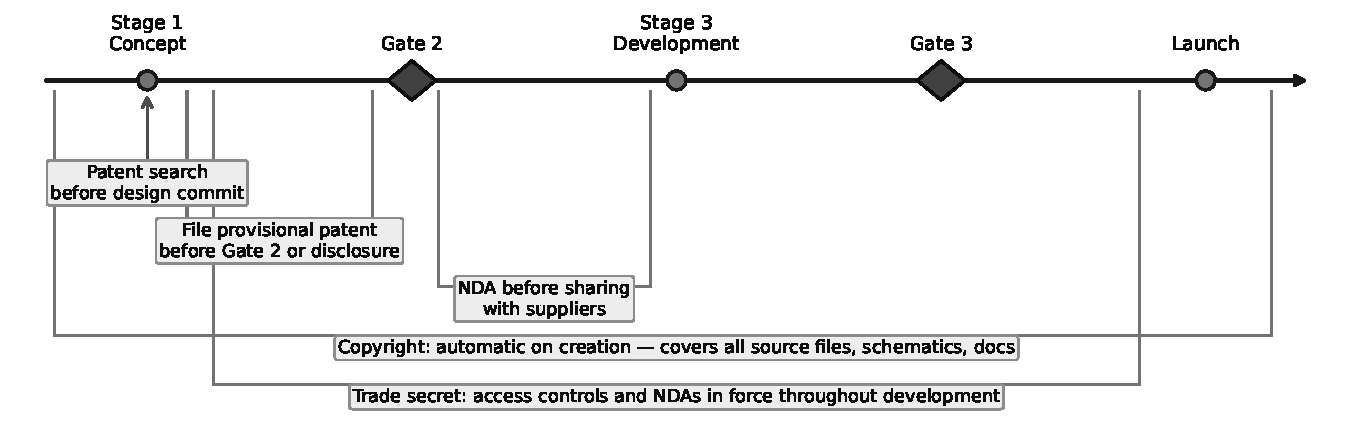
\includegraphics[width=0.92\textwidth]{chapters/15-ip/images/fig_02_ip_timeline}
  \caption{IP considerations mapped across the Stage-Gate timeline for the IoT
           robotic sorting subsystem.
           Diamond markers denote gates; circle markers denote stages.
           Each annotation below the timeline identifies the appropriate
           moment for the corresponding IP action.}
  \label{fig:ch15-ip-timeline}
\end{figure}

The running example system comprises custom AI inference firmware, a custom analog
sensor array design, an MQTT protocol implementation, and standard mechanical
components.
At Stage~3/4, the team should conduct the following IP audit:

\begin{enumerate}
  \item \textbf{Patent-eligible.}
        The custom sensor-array geometry combined with the AI classification
        algorithm constitutes a candidate for utility patent protection.
        The combination is novel (no prior art found for this specific geometry
        paired with this classification approach) and non-obvious (the performance
        improvement is not predictable from either component alone).
        The team should engage a patent agent to assess patentability and draft
        a provisional application before the next public disclosure.

  \item \textbf{Trade secret.}
        The trained model weights and the training dataset are best protected as
        trade secrets.
        They cannot be recovered by reverse-engineering the firmware binary,
        they derive substantial economic value from their secrecy, and the cost
        of re-creating them is high.
        Required controls: encrypted storage, access-logged retrieval, training
        pipeline under version control in a private repository, and NDAs with any
        external party who receives model outputs.

  \item \textbf{Copyright (automatic).}
        All firmware source files, schematic files, PCB layout files, simulation
        scripts, and this documentation are protected by copyright from the moment
        of creation.
        The team does not need to file anything; they should, however, ensure that
        the employment agreements of all contributing team members contain IP
        assignment clauses so that the employer holds a consolidated copyright, not
        a patchwork of individual ownership claims.

  \item \textbf{Trademark.}
        Not applicable at prototype stage.
        The product has not launched commercially, so there is no mark in use.
        The team should select a candidate product name now and run a clearance
        search against CIPO and USPTO databases before investing in branding.

  \item \textbf{Before trade-show disclosure.}
        Before presenting the system at any public venue, the team must either
        file a provisional patent application covering the sensor-array and
        algorithm combination, or obtain signed NDAs from every attendee who will
        receive a technical briefing.
        In practice, a trade show cannot guarantee NDA coverage; the provisional
        filing is the only reliable protection.
\end{enumerate}

\paragraph{In Practice.}
A medical-device team at a university incubator demonstrated their novel implant
sensor geometry at a regional engineering conference six weeks before their
provisional patent application was ready to file.
A competitor's engineer attended the demonstration, took detailed photographs of
the poster, and filed a patent application on a closely related design three weeks
later.
When the university team finally filed, the competitor's earlier publication date
(the conference paper uploaded to the conference website) constituted prior art
that partially invalidated the university team's novelty claim.
The cost of the conference registration: \$400.
The cost of the resulting patent dispute: \$180,000 in legal fees over three
years, with a settlement that required the university team to license the
technology back from the competitor.
Filing the provisional application before the conference would have cost \$320 in
USPTO fees.

\paragraph{Common Pitfalls.}
\begin{itemize}
  \item \textbf{Public disclosure before filing.}
        Any public disclosure --- conference poster, pre-print, trade-show
        demonstration, social media post with technical detail --- starts a
        twelve-month grace period in the United States (no grace period in most
        other jurisdictions) after which the disclosure itself constitutes
        invalidating prior art.
        File the provisional before you disclose, not after.

  \item \textbf{Assuming employer tools means no IP assignment.}
        Using a personal laptop with employer-licensed software to solve a work
        problem does not move the work outside the employer's ownership claim.
        Scope of employment is determined by the subject matter and purpose of
        the work, not the physical location of the keyboard.

  \item \textbf{Skipping the NDA before showing a prototype.}
        A handshake and a verbal assurance that ``everything we discuss is
        confidential'' has no legal effect.
        An NDA is a written contract; the writing requirement is not a formality.
        Prepare a standard one-page mutual NDA template in advance, and make
        signing it the first step of every technical meeting with an external party.
\end{itemize}

% ─────────────────────────────────────────────────────────────────────────────
\section*{Try It Yourself}
\addcontentsline{toc}{section}{Try It Yourself}
\label{sec:ch15-try}
% ─────────────────────────────────────────────────────────────────────────────

A start-up builds a wearable ECG monitor with the following elements:
\begin{enumerate}
  \item[(a)] A custom electrode adhesive geometry that improves skin-contact
             impedance by 40\% compared to commercially available electrodes.
  \item[(b)] A proprietary signal-processing algorithm trained on 50,000
             de-identified patient records, achieving clinical-grade arrhythmia
             detection at a fraction of the compute cost of prior art.
  \item[(c)] Firmware written by an independent contractor under a fixed-price
             contract that states ``all work product belongs to the contractor,''
             with no IP assignment or licence provisions.
  \item[(d)] The brand name ``CardioSense,'' which the team has been using in
             investor presentations for six months.
\end{enumerate}

For each element, identify the most appropriate form of IP protection and state
one risk if that protection is not pursued.

% ─────────────────────────────────────────────────────────────────────────────
\section*{Review Questions}
\addcontentsline{toc}{section}{Review Questions}
\label{sec:ch15-review}
% ─────────────────────────────────────────────────────────────────────────────

\begin{enumerate}
  \item \textit{(conceptual)} Explain the trade-off between filing a patent and
        keeping a process as a trade secret.
        Under what conditions would you choose each?

  \item \textit{(conceptual)} A firmware developer working at a start-up claims
        personal ownership of code because they wrote it at home on weekends,
        but using work equipment and solving a work problem.
        Explain, using the employment IP doctrine, why this claim is unlikely
        to succeed.

  \item \textit{(applied)} Identify the most appropriate IP protection for each:
        \begin{enumerate}
          \item[(a)] a novel battery-charging circuit topology;
          \item[(b)] a customer list compiled over five years;
          \item[(c)] the source code for an embedded sensor driver;
          \item[(d)] the name ``SortBot Pro'' on a product label.
        \end{enumerate}

  \item \textit{(applied)} A team is about to show their prototype to a potential
        contract manufacturer.
        List three specific items that should be in the NDA and one item that an
        NDA typically does \emph{not} protect.

  \item \textit{(applied, multi-step)} A contractor is hired to design a custom
        PCB under a contract that states ``all work product belongs to the
        contractor.''
        The client later discovers the PCB contains a patentable improvement.
        Who owns the patent right?
        What should the contract have said instead, and at what stage should it
        have been negotiated?
\end{enumerate}

% ─────────────────────────────────────────────────────────────────────────────
\section*{Portfolio Entry}
\addcontentsline{toc}{section}{Portfolio Entry}
\label{sec:ch15-portfolio}
% ─────────────────────────────────────────────────────────────────────────────

Produce an IP checklist for your project with four sections:
\begin{enumerate}
  \item[(a)] \textit{Protectable elements} --- list each design element or feature
             that may be eligible for patent, trade secret, or copyright
             protection, with the recommended form of protection.
  \item[(b)] \textit{Ownership assignment} --- state who owns each element
             (employer, contractor, joint) and whether your employment or
             contractor agreement explicitly addresses it.
  \item[(c)] \textit{NDA requirement} --- identify every external party
             (supplier, manufacturer, advisor) who will see the prototype and
             state whether an NDA has been executed.
  \item[(d)] \textit{Prior-art search status} --- record the databases searched,
             search terms used, and any relevant prior art found.
\end{enumerate}
Submit this as Section~15 of your prototype documentation package.

% ─────────────────────────────────────────────────────────────────────────────
\section*{Chapter Summary}
\addcontentsline{toc}{section}{Chapter Summary}
\label{sec:ch15-summary}
% ─────────────────────────────────────────────────────────────────────────────

Intellectual property protection is not a legal afterthought reserved for large
companies with dedicated counsel.
It is a set of active, time-sensitive choices that engineering teams must make at
specific moments in the development timeline --- before a public disclosure, before
showing a prototype to a supplier, before signing a contractor agreement, before
committing to a product name.

The four main categories of protection --- \textbf{patent}, \textbf{trade
secret}, \textbf{copyright}, and \textbf{trademark} --- cover different kinds of
assets, operate through different legal mechanisms, and involve different
trade-offs between disclosure and exclusivity.
Copyright arises automatically; the others require deliberate action.
Ownership in employment defaults to the employer for work within the scope of
employment; in contracting, it defaults to the contractor unless an explicit
assignment clause provides otherwise.
NDAs are the primary instrument for sharing designs with external parties without
sacrificing trade-secret protection or novelty.

The procedural habits this chapter asks you to form are simple:
conduct a prior-art search before committing to a design direction;
file a provisional patent application or obtain NDAs before any public disclosure;
read your employment agreement and understand what you own and what your employer
owns; and engage a patent agent at the first sign that your design may be
commercially significant.

Chapter~16 compiles every section produced since Chapter~1 into the coherent
portfolio that Gate~3 requires, integrating the IP checklist from Section~15,
the version-controlled design history from Chapter~13, the validation records
from Chapter~14, and the economic analysis from Chapter~12 into a single,
auditable package that a gate reviewer can evaluate with confidence.
